\documentclass[a4paper,11pt]{article}

\usepackage[latin1]{inputenc}
\usepackage[italian]{babel}
\usepackage[T1]{fontenc}

%immagini
\usepackage{xcolor}
\usepackage{graphicx}

%tabelle
\usepackage{array}
\usepackage{tabularx}
\usepackage{longtable}
\usepackage{booktabs}
\usepackage{multirow}
\usepackage{colortbl}

%collegamenti ipertestuali
\usepackage{hyperref}
\hypersetup{colorlinks=true, linkcolor=blue, urlcolor=blue}


\title{Macchina Astratta}
\author{Andrea Zanelli}
\date{\today}


% INIZIO DOCUMENTO *************************************************************
\begin{document}

% PRIMA PAGINA *****************************************************************
\maketitle
\pagebreak

% INDICE ***********************************************************************
\tableofcontents
\pagebreak

% INTRODUZIONE *****************************************************************
\section{Introduzione}
\label{sec:introduzione}
In questo documento viene elencato e descritto l'instruction set della macchina astratta e viene illustrata la sua struttura di funzionamento. In entrambi i casi \`e basata sulla Java Virtual Machine (JVM). Per l'instruction set \`e stato preso un sottoinsieme di quello della JVM, percui un programma funzionante su questa macchina astratta funziona anche sulla JVM, traducendo per\`o gli mnemonici in bytecode con un assembler come, per esempio, l'Oolong scritto da Joshua Engel. La struttura, in modo simile alla JVM, \`e composta da uno stack di sistema, in cui vengono messi i record di attivazione (RdA) di ogni funzione che viene eseguita, e da una area-programma dove vengono memorizzate le istruzioni da eseguire. Ogni RdA \`e quindi composto da un program counter (PC) che punta all'istruzione da eseguire, da uno stack degli operandi e da un array delle variabili locali.

%\pagebreak

% DIRETTIVE ********************************************************************
\section{Direttive}
\label{sec:direttive}
Le direttive vengono utilizzate per definire l'inizio e la fine del programma, per dichirare le variabili globali e le funzioni.

\subsection{Tabella direttive}
\label{sec:tabella_direttive}
{\footnotesize
\begin{tabularx}{\columnwidth}{l X}
\toprule
\rowcolor[gray]{0.9}
  \textbf{Direttiva} &
  \textbf{Descrizione} \\
\toprule
  \texttt{.class~public Main} &
  Inizio del programma \\
\midrule
  \texttt{.super~java/lang/Object} &
  Inizio del programma (da mettere subito dopo \texttt{.class~public Main}) \\
\midrule
  \texttt{.end~class} &
  Fine del programma \\
\midrule
  \texttt{.field public static \textit{f} \textit{d}} &
  Variabile globale \texttt{\textit{f}} \\
\midrule
  \texttt{.method public static \textit{m} \textit{d}} &
  Inizio della funzione \texttt{\textit{m}} \\
\midrule
  \texttt{.end method} &
  Fine della funzione \\
\bottomrule
\end{tabularx}
} % end \footnotesize

\subsection{Inizio e fine programma}
Un programma ha inizio dopo le due seguenti direttive
\begin{quote}
  \texttt{.class public Main} \\
  \texttt{.super java/lang/Object}
\end{quote}
e finisce con la direttiva
\begin{quote}
  \texttt{.end class}
\end{quote}
Fra queste direttive di inizio e fine del programma vengono definite le funzioni e le variabili globali. Ogni scritta prima di \texttt{.class~public Main} e dopo \texttt{.end~class} \`e considerata errore.
\subsubsection*{Esempio}
\begin{verbatim}
.class public Main
.super java/lang/Object
  ; funzioni e variabili globali
.end class
\end{verbatim}

\subsection{Variabili globali}
Le variabili globali si definiscono con la direttiva
\begin{quote}
  \texttt{.field public static \textit{fieldname} \textit{descriptor}}
\end{quote}
dove \texttt{\textit{fieldname}} \`e il nome della variabile e \texttt{\textit{descriptor}} \`e il tipo della variabile (vedere tabella dei tipi: \ref{sec:tabella_tipi}).
\subsubsection*{Esempio}
Variabile globale di nome \texttt{numberOfElements} e di tipo \texttt{int}:
\begin{verbatim}
.field public static numberOfElements I
\end{verbatim}

\subsection{Funzioni}
Per la dichiarazione di una funzione e per indicarne l'inizio si usa la direttiva
\begin{quote}
  \texttt{.method public static \textit{methodname} \textit{descriptor}}
\end{quote}
dove \texttt{\textit{methodname}} \`e il nome della funzione e \texttt{\textit{decriptor}} descrive gli argomenti e il tipo di ritorno della funzione (vedere la tabella dei tipi: \ref{tab:tabella_tipi}). \\
Per indicare la fine della definizione della funzione si usa la direttiva
\begin{quote}
  \texttt{.end method}
\end{quote}
Fra le direttive \texttt{.method} e \texttt{.end~method} vi sono le istruzioni della funzione (vedere le tabelle delle istruzioni nel paragrafo \ref{sec:tabelle_istruzioni}).
\subsubsection*{Esempio}
Funzione di nome \texttt{icalc} che prende come argomenti quattro interi e ritorna un intero
\begin{verbatim}
.method public static icalc(IIII)I
  ; serie di istruzioni
.end method
\end{verbatim}

\subsection{Funzione inizializzatore}
Se esiste \`e la prima funzione ad essere eseguita ed \`e utilizzata per inizializzare le variabili globali prima di eseguire la funzione principale; ha nome \texttt{<clinit>}, non prende argomenti e ha tipo di ritorno void:
\begin{quote}
  \texttt{.method public static <clinit> ()V}
\end{quote}
Se nel testo del programma non c'\`e la funzione \texttt{<clinit>} viene eseguita direttamente la funzione principale.
\subsubsection*{Esempio}
\begin{verbatim}
.method public static <clinit> ()V
  ; serie di istruzioni per inizializzare
  ; le variabili globali
  return
.end method
\end{verbatim}

\subsection{Funzione principale}
\`E la funzione principale, la prima ad essere eseguita (se non esiste la funzione inizializzatore) e da cui inizia il programma, ha nome \texttt{main}:
\begin{quote}
  \texttt{.method public static main([Ljava/lang/String;)V}
\end{quote}
Se nel testo del programma non c'\`e la funzione \texttt{main} viene segnalato un errore e il programma non pu\`o essere eseguito.
\subsubsection*{Esempio}
\begin{verbatim}
.method public static main([Ljava/lang/String;)V
  return
.end method
\end{verbatim}

%\pagebreak

% TIPI *************************************************************************
\section{Tipi}
\label{sec:tipi}
Nella macchina astratta sono implementati i seguenti tipi:
\begin{itemize}
  \item \texttt{int}
  \item \texttt{long}
  \item \texttt{short}
  \item \texttt{char}
\end{itemize}
Si possono usare inoltre le ``costanti stringa'' (\texttt{String}) con le seguenti caratteristiche: sono racchiuse da virgolette (''), con l'istruzione \texttt{ldc\_w ''stringa''} si mette la costante stringa in cima allo stack, si possono stampare su output con la funzione di stampa e argomento \texttt{Ljava/lang/String;}, si possono leggere da standard input terminate da un a-capo, \textbf{non} vi sono altre istruzioni di alcun tipo sulle stringhe, \textbf{non} si possono assegnare a variabili globali o locali, \textbf{non} possono essere passate come parametro a funzioni o usate come valore di ritorno.

\subsection{Tabella tipi}
\label{sec:tabella_tipi}
Qui sotto la tabella contenente i tipi disponibili nel linguaggio della macchina astratta, con il descrittore corrispondente, cio\`e il simbolo che identifica il tipo, da mettere nelle funzioni (per gli argomenti e il tipo di ritorno) e nelle variabili globali (per il tipo di variabile).

{\footnotesize
\begin{center}
\begin{tabular}{p{2cm} l}
\toprule
\rowcolor[gray]{0.9}
  \textbf{Tipo} &
  \textbf{Descrittore} \\
\toprule
  \texttt{char} &
  \texttt{C} \\
%\midrule
  \texttt{int} &
  \texttt{I} \\
%\midrule
  \texttt{long} &
  \texttt{J} \\
%\midrule
  \texttt{short} &
  \texttt{S} \\
%\midrule
  \texttt{void} &
  \texttt{V} \\
\bottomrule
\end{tabular}
\label{tab:tabella_tipi}
\end{center}
} % end \footnotesize

\subsection{Rappresentazioni e conversioni}
\label{sec:rappresentazioni_e_conversioni}
Le conversioni da un tipo pi\`u piccolo ad uno pi\`u grande (promozioni), per esempio da \texttt{int} a \texttt{long}, sono fatte normalmente, mantenendo inalterato il valore. Le conversioni da un tipo pi\`u grande, diciamo \texttt{T}, ad uno pi\`u piccolo, diciamo \texttt{t}, per esempio da \texttt{int} a \texttt{short}, vengono fatte nel seguente modo: se il valore di \texttt{T} \`e compreso tra i valori possibili di \texttt{t}, allora la conversione avviene normalmente; se il valore di \texttt{T} \`e maggiore del pi\`u grande valore di \texttt{t}, allora si ricomincia (in modo ciclico) dal valore pi\`u piccolo di \texttt{t}, quindi se, ad esempio, si vuol convertire l'\texttt{int} +32769 in un \texttt{short}, prender\`a il valore -32767, allo stesso modo l'\texttt{int} 98304 prender\`a il valore -32768; se il valore di \texttt{T} \`e minore del pi\`u piccolo valore di \texttt{t}, allora si ricomincia (in modo ciclico) dal valore pi\`u grande di \texttt{t}, quindi se, ad esempio, si vuol convertire l'\texttt{int} -32769 in un \texttt{short}, prender\`a il valore +32767.

\subsubsection*{Tabella rappresentazioni}
\label{sec:tabella_rappresentazioni}
Qui sotto la tabella con la rappresentazione binaria ed i valori che pu\`o assumere ogni tipo.

{\footnotesize
\begin{center}
\begin{tabular}{l l r r}
\toprule
\rowcolor[gray]{0.9}
  \textbf{Tipo} &
  \textbf{Rappresentazione} &
  \textbf{da} &
  \textbf{a} \\
\toprule
  \texttt{int} &
  32 bit, con segno &
  -2.147.483.648 &
  +2.147.483.647 \\
%\midrule
  \texttt{short} &
  16 bit, con segno &
  -32.768 &
  +32.767 \\
%\midrule
  \texttt{long} &
  64 bit, con segno &
  -$2^{63}$ &
  $+2^{63}-1$ \\
%\midrule
  \texttt{char} &
  16 bit, senza segno &
  0 &
  +65.535 \\
\bottomrule
\end{tabular}
\end{center}
} % end \footnotesize

I tipi \texttt{int}, \texttt{short} e \texttt{char} occupano uno slot sullo stack ed un solo registro nelle variabili locali, il tipo \texttt{long} occupa due slot sullo stack e due registri (consecutivi) nelle variabili locali.

%\pagebreak

% ISTRUZIONI *******************************************************************
\section{Istruzioni}
\label{sec:istruzioni}
Chiavi di lettura per le istruzioni:
{\footnotesize
\begin{longtable}{>{\ttfamily}p{1cm} p{9.5cm}}
\toprule
  a &
  Slot in cima allo stack (top). Pu\`o contenere \texttt{int} o costanti stringa \\

  b &
  Secondo slot dello stack. Pu\`o contenere \texttt{int} o costanti stringa \\

  c &
  Terzo slot dello stack. Pu\`o contenere \texttt{int} o costanti stringa \\

  d &
  Quarto slot dello stack. Pu\`o contenere \texttt{int} o costanti stringa \\

  ab &
  Primo e secondo slot dello stack. Usato per tipi \texttt{long} \\

  cd &
  Terzo e quarto slot dello stack. Usato per tipi \texttt{long} \\
\bottomrule
\end{longtable}
} % end \footnotesize


\subsection{Tabelle istruzioni}
\label{sec:tabelle_istruzioni}
Di seguito tutte le istruzioni divise per categoria con una breve descrizione. Per maggiori dettagli si rimanda al paragrafo \ref{sec:dettagli_istruzioni}.

\subsubsection*{Aritmetiche}
\label{sec:aritmetiche}
{\footnotesize
\begin{longtable}{p{2cm} p{2cm} p{6.5cm}}
\toprule
\rowcolor[gray]{0.9}
  \textbf{Istruzione} &
  \textbf{Argomenti} &
  \textbf{Descrizione} \\
\toprule
\endhead
  \texttt{iadd} &
  &
  Somma \texttt{int} (\texttt{b+a})  \\

  \texttt{idiv} &
  &
  Divisione \texttt{int} (\texttt{b/a}) \\

  \texttt{imul} &
  &
  Moltiplicazione \texttt{int} (\texttt{b*a}) \\

  \texttt{ineg} &
  &
  Negazione \texttt{int} (\texttt{-a}) \\

  \texttt{irem} &
  &
  Resto divisione \texttt{int} (\texttt{b\%a}) \\

  \texttt{ishl} &
  &
  Shift \texttt{int} a sinistra (\texttt{b << a}) \\

  \texttt{ishr} &
  &
  Shift \texttt{int} a destra (\texttt{b >> a}) \\

  \texttt{isub} &
  &
  Sottrazione \texttt{int} (\texttt{b-a}) \\

  \texttt{ladd} &
  &
  Somma \texttt{long} (\texttt{cd+ab})  \\

  \texttt{ldiv} &
  &
  Divisione \texttt{long} (\texttt{cd/ab}) \\

  \texttt{lmul} &
  &
  Moltiplicazione \texttt{long} (\texttt{cd*ab}) \\

  \texttt{lneg} &
  &
  Negazione \texttt{long} (\texttt{-ab}) \\

  \texttt{lrem} &
  &
  Resto divisione \texttt{long} (\texttt{cd\%ab}) \\

  \texttt{lshl} &
  &
  Shift \texttt{long} a sinistra (\texttt{bc << a}) \\

  \texttt{lshr} &
  &
  Shift \texttt{long} a destra (\texttt{bc >> a}) \\

  \texttt{lsub} &
  &
  Sottrazione \texttt{long} (\texttt{cd-ab}) \\
\bottomrule
\end{longtable}
} % end \footnotesize

\subsubsection*{Costanti}
\label{sec:costanti}
{\footnotesize
\begin{longtable}{p{2cm} p{2cm} p{6.5cm}}
\toprule
\rowcolor[gray]{0.9}
  \textbf{Istruzione} &
  \textbf{Argomenti} &
  \textbf{Descrizione} \\
\toprule
\endhead
  \texttt{ldc\_w} &
  \texttt{x} &
  Mette \texttt{x} in cima allo stack (\texttt{int} o \texttt{String})  \\
  
  \texttt{ldc2\_w} &
  \texttt{x} &
  Mette \texttt{x} in cima allo stack (\texttt{long})  \\
  
  \texttt{sipush} &
  \texttt{n} &
  Mette \texttt{n} in cima allo stack (\texttt{short})  \\
\bottomrule
\end{longtable}
} % end \footnotesize

\subsubsection*{Controllo}
\label{sec:controllo}
{\footnotesize
\begin{longtable}{p{2cm} p{2cm} p{6.5cm}}
\toprule
\rowcolor[gray]{0.9}
  \textbf{Istruzione} &
  \textbf{Argomenti} &
  \textbf{Descrizione} \\
\toprule
\endhead
  \texttt{goto} &
  \texttt{label} &
  Salta all'istruzione contrassegnata con \texttt{label} \\
  
  \texttt{if\_icmpeq} &
  \texttt{label} &
  Salta a \texttt{label} se \texttt{b == a} \\
  
  \texttt{if\_icmpge} &
  \texttt{label} &
  Salta a \texttt{label} se \texttt{b >= a} \\
  
  \texttt{if\_icmpgt} &
  \texttt{label} &
  Salta a \texttt{label} se \texttt{b > a} \\
  
  \texttt{if\_icmple} &
  \texttt{label} &
  Salta a \texttt{label} se \texttt{b <= a} \\
  
  \texttt{if\_icmplt} &
  \texttt{label} &
  Salta a \texttt{label} se \texttt{b < a} \\
  
  \texttt{if\_icmpne} &
  \texttt{label} &
  Salta a \texttt{label} se \texttt{b != a} \\
  
  \texttt{ifeq} &
  \texttt{label} &
  Salta a \texttt{label} se \texttt{a == 0} \\
  
  \texttt{ifge} &
  \texttt{label} &
  Salta a \texttt{label} se \texttt{a >= 0} \\
  
  \texttt{ifgt} &
  \texttt{label} &
  Salta a \texttt{label} se \texttt{a > 0} \\
  
  \texttt{ifle} &
  \texttt{label} &
  Salta a \texttt{label} se \texttt{a <= 0} \\
  
  \texttt{iflt} &
  \texttt{label} &
  Salta a \texttt{label} se \texttt{a < 0} \\
  
  \texttt{ifne} &
  \texttt{label} &
  Salta a \texttt{label} se \texttt{a != 0} \\
  
  \texttt{ireturn} &
  &
  Ritorna un \texttt{int} alla funzione chiamante \\
  
  \texttt{lcmp} &
  &
  Confronto tra \texttt{long} \\
  
  \texttt{lreturn} &
  &
  Ritorna un \texttt{long} alla funzione chiamante \\
  
  \texttt{nop} &
  &
  Non fa' niente \\
  
  \texttt{return} &
  &
  Ritorna al metodo chiamante \\
\bottomrule
\end{longtable}
} % end \footnotesize

\subsubsection*{Conversione di tipi}
\label{sec:conversione_di_tipi}
{\footnotesize
\begin{longtable}{p{2cm} p{2cm} p{6.5cm}}
\toprule
\rowcolor[gray]{0.9}
  \textbf{Istruzione} &
  \textbf{Argomenti} &
  \textbf{Descrizione} \\
\toprule
\endhead
  \texttt{i2c} &
  &
  Converte l'\texttt{int} in \texttt{a} in \texttt{char} \\

  \texttt{i2s} &
  &
  Converte l'\texttt{int} in \texttt{a} in \texttt{short} \\
  
  \texttt{i2l} &
  &
  Converte l'\texttt{int} in \texttt{a} in \texttt{long} \\
  
  \texttt{l2i} &
  &
  Converte il \texttt{long} in \texttt{ab} in \texttt{int} \\
\bottomrule
\end{longtable}
} % end \footnotesize

\subsubsection*{Operazioni sullo stack}
\label{sec:operazioni_sullo_stack}
{\footnotesize
\begin{longtable}{p{2cm} p{2cm} p{6.5cm}}
\toprule
\rowcolor[gray]{0.9}
  \textbf{Istruzione} &
  \textbf{Argomenti} &
  \textbf{Descrizione} \\
\toprule
\endhead
  \texttt{dup} &
  &
  Duplica \texttt{a} \\

  \texttt{dup2} &
  &
  Duplica \texttt{ab} \\
  
  \texttt{pop} &
  &
  Rimuove \texttt{a} \\
  
  \texttt{pop2} &
  &
  Rimuove \texttt{ab} \\
  
  \texttt{swap} &
  &
  Scambia \texttt{a} con \texttt{b} \\
\bottomrule
\end{longtable}
} % end \footnotesize

\subsubsection*{Funzioni e variabili globali}
\label{sec:funzioni_e_varibili_globali}
{\footnotesize
\begin{longtable}{p{2cm} p{2cm} p{6.5cm}}
\toprule
\rowcolor[gray]{0.9}
  \textbf{Istruzione} &
  \textbf{Argomenti} &
  \textbf{Descrizione} \\
\toprule
\endhead
  \texttt{getstatic} &
  \texttt{Main/\textit{f} \textit{d}} &
  Mette sullo stack \texttt{\textit{f d}} (variabile globale) \\

  \texttt{invokestatic} &
  \texttt{Main/\textit{m} \textit{d}} &
  Chiama la funzione \texttt{\textit{m d}} \\
  
  \texttt{putstatic} &
  \texttt{Main/\textit{f} \textit{d}} &
  Memorizza in \texttt{\textit{f d}} (variabile globale) \\
\bottomrule
\end{longtable}
} % end \footnotesize

\subsubsection*{Variabili}
\label{sec:variabili}
{\footnotesize
\begin{longtable}{p{2cm} p{2cm} p{6.5cm}}
\toprule
\rowcolor[gray]{0.9}
  \textbf{Istruzione} &
  \textbf{Argomenti} &
  \textbf{Descrizione} \\
\toprule
\endhead
  \texttt{iload} &
  \texttt{n} &
  Mette sullo stack la variabile locale \texttt{n} (\texttt{int}) \\

  \texttt{istore} &
  \texttt{n} &
  Mette \texttt{a} nella variabile locale \texttt{n}\\
  
  \texttt{lload} &
  \texttt{n} &
  Mette sullo stack la variabile locale \texttt{n} (\texttt{long}) \\
  
  \texttt{lstore} &
  \texttt{n} &
  Mette \texttt{ab} nella variabile locale \texttt{n}\\
\bottomrule
\end{longtable}
} % end \footnotesize


\subsection{Dettagli istruzioni}
\label{sec:dettagli_istruzioni}
\begin{description}
  \item[\texttt{dup}:] duplica e mette sullo stack il valore di tipo \texttt{int} in cima allo stack (\texttt{a}).

  \item[\texttt{dup2}:] duplica e mette sullo stack il valore di tipo \texttt{long} in cima allo stack (\texttt{ab}).

  \item[\texttt{getstatic Main/\textit{f} \textit{d}}:] mette in cima allo stack il valore della variabile globale di nome \texttt{\textit{f}} e tipo \texttt{\textit{d}} (vedere la tabella dei tipi: \ref{sec:tabella_tipi}).

  \item[\texttt{goto label}:] salta all'istruzione etichettata con \texttt{label}.

  \item[\texttt{i2c}:] preleva l'\texttt{int} in cima allo stack (\texttt{a}), lo converte in \texttt{char} e mette il risultato in cima allo stack.

  \item[\texttt{i2l}:] preleva l'\texttt{int} in cima allo stack (\texttt{a}), lo converte in \texttt{long} e mette il risultato in cima allo stack.

  \item[\texttt{i2s}:] preleva l'\texttt{int} in cima allo stack (\texttt{a}), lo converte in \texttt{short} e mette il risultato in cima allo stack.

  \item[\texttt{iadd}:] preleva i primi due \texttt{int} in cima allo stack (\texttt{a} e \texttt{b}), esegue la somma tra il secondo e il primo (\texttt{b+a}), mette il risultato (\texttt{int}) sullo stack.

  \item[\texttt{idiv}:] preleva i primi due \texttt{int} in cima allo stack (\texttt{a} e \texttt{b}), esegue la divisione tra il secondo e il primo (\texttt{b/a}), mette il risultato (\texttt{int}) sullo stack.

  \item[\texttt{if\_icmpeq label}:] preleva i primi due \texttt{int} in cima allo stack (\texttt{a} e \texttt{b}), se il secondo \`e uguale al primo (\texttt{b == a}) salta all'istruzione etichettata con \texttt{label}, altrimenti esegue l'istruzione successiva.

  \item[\texttt{if\_icmpge label}:] preleva i primi due \texttt{int} in cima allo stack (\texttt{a} e \texttt{b}), se il secondo \`e maggiore o uguale al primo (\texttt{b >= a}) salta all'istruzione etichettata con \texttt{label}, altrimenti esegue l'istruzione successiva.

  \item[\texttt{if\_icmpgt label}:] preleva i primi due \texttt{int} in cima allo stack (\texttt{a} e \texttt{b}), se il secondo \`e maggiore del primo (\texttt{b > a}) salta all'istruzione etichettata con \texttt{label}, altrimenti esegue l'istruzione successiva.

  \item[\texttt{if\_icmple label}:] preleva i primi due \texttt{int} in cima allo stack (\texttt{a} e \texttt{b}), se il secondo \`e minore o uguale al primo (\texttt{b <= a}) salta all'istruzione etichettata con \texttt{label}, altrimenti esegue l'istruzione successiva.

  \item[\texttt{if\_icmplt label}:] preleva i primi due \texttt{int} in cima allo stack (\texttt{a} e \texttt{b}), se il secondo \`e minore del primo (\texttt{b < a}) salta all'istruzione etichettata con \texttt{label}, altrimenti esegue l'istruzione successiva.

  \item[\texttt{if\_icmpne label}:] preleva i primi due \texttt{int} in cima allo stack (\texttt{a} e \texttt{b}), se il secondo \`e diverso dal primo (\texttt{b != a}) salta all'istruzione etichettata con \texttt{label}, altrimenti esegue l'istruzione successiva.

  \item[\texttt{ifeq label}:] preleva l'\texttt{int} in cima allo stack (\texttt{a}), se \`e uguale a zero (\texttt{a == 0}) salta all'istruzione etichettata con \texttt{label}, altrimenti esegue l'istruzione successiva.

  \item[\texttt{ifge label}:] preleva l'\texttt{int} in cima allo stack (\texttt{a}), se \`e maggiore o uguale a zero (\texttt{a >= 0}) salta all'istruzione etichettata con \texttt{label}, altrimenti esegue l'istruzione successiva.

  \item[\texttt{ifgt label}:] preleva l'\texttt{int} in cima allo stack (\texttt{a}), se \`e maggiore di zero (\texttt{a > 0}) salta all'istruzione etichettata con \texttt{label}, altrimenti esegue l'istruzione successiva.

  \item[\texttt{ifle label}:] preleva l'\texttt{int} in cima allo stack (\texttt{a}), se \`e minore o uguale a zero (\texttt{a <= 0}) salta all'istruzione etichettata con \texttt{label}, altrimenti esegue l'istruzione successiva.

  \item[\texttt{iflt label}:] preleva l'\texttt{int} in cima allo stack (\texttt{a}), se \`e minore di zero (\texttt{a < 0}) salta all'istruzione etichettata con \texttt{label}, altrimenti esegue l'istruzione successiva.

  \item[\texttt{ifne label}:] preleva l'\texttt{int} in cima allo stack (\texttt{a}), se \`e diverso da zero (\texttt{a != 0}) salta all'istruzione etichettata con \texttt{label}, altrimenti esegue l'istruzione successiva.

  \item[\texttt{iload n}:] mette in cima allo stack l'\texttt{int} memorizzato nella variabile locale \texttt{n}.

  \item[\texttt{imul}:] preleva i primi due \texttt{int} in cima allo stack (\texttt{a} e \texttt{b}), esegue il prodotto tra il secondo e il primo (\texttt{b*a}), mette il risultato (\texttt{int}) sullo stack.

  \item[\texttt{ineg}:] preleva l'\texttt{int} in cima allo stack (\texttt{a}), lo nega (\texttt{-a}) e mette il risultato sullo stack.

  \item[\texttt{invokestatic Main/\textit{m} \textit{d}}:] chiama la funzione di nome \texttt{\textit{m}} con descrittore \texttt{\textit{d}} (il descrittore contiene i tipi degli argomenti e il tipo di ritorno della funzione, vedere la tabella dei tipi: \ref{sec:tabella_tipi}) passandogli come parametri (se previsti dalla funzione) i valori sullo stack, in modo che il valore in cima allo stack corrisponde all'ultimo parametro richiesto dalla funzione, il secondo nello stack corrisponde al penultimo parametro, e cos\`i via. Nel corpo della funzione chiamata, i parametri passati vengono inseriti nelle prime variabili locali, quindi il primo parametro sar\`a nella variabile locale \texttt{0}, il secondo in \texttt{1} (supponendo che il primo occupava un solo posto nelle variabili), e cos\`i via. Al termine dell'esecuzione della funzione, se ha un valore di ritorno viene messo in cima allo stack del chiamante.

  \item[\texttt{irem}:] preleva i primi due \texttt{int} in cima allo stack (\texttt{a} e \texttt{b}), calcola il resto della divisione tra il secondo e il primo (\texttt{b\%a}) e mette il risultato (\texttt{int}) sullo stack.

  \item[\texttt{ireturn}:] preleva l'\texttt{int} in cima allo stack (\texttt{a}), termina l'esecuzione della funzione, torna il controllo alla funzione chiamante e mette l'\texttt{int} in cima allo stack. Da utilizzare nelle funzioni che hanno come tipo di ritorno \texttt{I}, \texttt{S} o \texttt{C}.

  \item[\texttt{ishl}:] preleva i primi due \texttt{int} in cima allo stack (\texttt{a} e \texttt{b}), calcola lo shift a sinistra del secondo valore con il primo (\texttt{b} << \texttt{a}) e mette il risultato (\texttt{int}) sullo stack.

  \item[\texttt{ishr}:] preleva i primi due \texttt{int} in cima allo stack (\texttt{a} e \texttt{b}), calcola lo shift a destra del secondo valore con il primo (\texttt{b} >> \texttt{a}) e mette il risultato (\texttt{int}) sullo stack.

  \item[\texttt{istore n}:] preleva l'\texttt{int} in cima allo stack (\texttt{a}), e memorizza il valore nella variabile locale \texttt{n}.

  \item[\texttt{isub}:] preleva i primi due \texttt{int} in cima allo stack (\texttt{a} e \texttt{b}), esegue la sottrazione tra il secondo e il primo (\texttt{b-a}), mette il risultato (\texttt{int}) sullo stack.

  \item[\texttt{l2i}:] preleva il \texttt{long} in cima allo stack \texttt{ab}, lo converte in \texttt{int} e mette il risultato in cima allo stack.

  \item[\texttt{ladd}:] preleva i primi due \texttt{long} in cima allo stack (\texttt{ab} e \texttt{cd}), esegue la somma tra il primo e il secondo (\texttt{ab+cd}) e mette il risultato (\texttt{long}) sullo stack.

  \item[\texttt{lcmp}:] preleva i primi due \texttt{long} in cima allo stack (\texttt{ab} e \texttt{cd}), li confronta, e mette sullo stack il numero 1 (di tipo \texttt{int}) se il secondo valore \`e maggiore del primo (\texttt{cd > ab}), -1 se il secondo \`e minore del primo (\texttt{cd < ab}), 0 se i due valori sono uguali (\texttt{cd == ab}).

  \item[\texttt{ldc\_w x}:] mette in cima allo stack la costante \texttt{x} di tipo \texttt{int} o di tipo \texttt{String} (stringa tra virgolette). Se \texttt{x} \`e di tipo \texttt{int} dev'essere un numero intero compreso tra i valori rappresentati nella tabella dei tipi \ref{sec:tabella_rappresentazioni} a pagina \pageref{sec:tabella_rappresentazioni} (nella riga \texttt{int}). Se \texttt{x} \`e di tipo \texttt{String} dev'essere una stringa valida racchiusa tra virgolette.

  \item[\texttt{ldc2\_w x}:] mette in cima allo stack la costante \texttt{x} di tipo \texttt{long}. La costante \texttt{x} dev'essere un numero intero compreso tra i valori rappresentati nella tabella dei tipi \ref{sec:tabella_rappresentazioni} a pagina \pageref{sec:tabella_rappresentazioni} (nella riga \texttt{long}).

  \item[\texttt{ldiv}:] preleva i primi due \texttt{long} in cima allo stack (\texttt{ab} e \texttt{cd}), esegue la divisione tra il secondo e il primo (\texttt{cd/ab}) e mette il risultato (\texttt{long}) sullo stack.

  \item[\texttt{lload n}:] mette in cima allo stack il \texttt{long} memorizzato nella variabile locale \texttt{n}.

  \item[\texttt{lmul}:] preleva i primi due \texttt{long} in cima allo stack (\texttt{ab} e \texttt{cd}), esegue il prodotto tra il secondo e il primo (\texttt{cd*ab}) e mette il risultato (\texttt{long}) sullo stack.

  \item[\texttt{lneg}:] preleva il \texttt{long} in cima allo stack (\texttt{ab}), lo nega (\texttt{-ab}) e mette il risultato sullo stack.

  \item[\texttt{lrem}:] preleva i primi due \texttt{long} in cima allo stack (\texttt{ab} e \texttt{cd}), calcola il resto della divisione tra il secondo e il primo (\texttt{cd\%ab}) e mette il risultato (\texttt{long}) sullo stack.

  \item[\texttt{lreturn}:] preleva il \texttt{long} in cima allo stack (\texttt{ab}), termina l'esecuzione della funzione, torna il controllo alla funzione chiamante e mette il \texttt{long} in cima allo stack. Da utilizzare nelle funzioni che hanno come tipo di ritorno \texttt{J}.

  \item[\texttt{lshl}:] preleva un \texttt{int} e un \texttt{long} dallo stack (\texttt{a} e \texttt{bc}), calcola lo shift a sinistra del valore di tipo \texttt{long} (\texttt{bc} << \texttt{a}) e mette il risultato (\texttt{long}) sullo stack.

  \item[\texttt{lshr}] preleva un \texttt{int} e un \texttt{long} dallo stack (\texttt{a} e \texttt{bc}), calcola lo shift a destra del valore di tipo \texttt{long} (\texttt{bc} >> \texttt{a}) e mette il risultato (\texttt{long}) sullo stack.

  \item[\texttt{lstore n}:] preleva il \texttt{long} in cima allo stack (\texttt{ab}), e memorizza il valore nella variabile locale \texttt{n} (\textbf{nota}: un long occupa due posizioni nelle variabili locali).

  \item[\texttt{lsub}:] preleva i primi due \texttt{long} in cima allo stack (\texttt{ab} e \texttt{cd}), esegue la sottrazione tra il secondo e il primo (\texttt{cd-ab}) e mette il risultato (\texttt{long}) sullo stack.

  \item[\texttt{nop}:] non fa niente.

  \item[\texttt{pop}:] toglie il valore nel primo slot in cima allo stack (\texttt{a}).

  \item[\texttt{pop2}:] toglie i valori nei primi due slot in cima allo stack (\texttt{ab}).

  \item[\texttt{putstatic Main/\textit{f} \textit{d}}:] mette nella variabile globale di nome \texttt{\textit{f}} e tipo \texttt{\textit{d}} il valore in cima allo stack.

  \item[\texttt{return}:] interrompe l'esecuzione della funzione e torna il controllo alla funzione chiamante. Da utilizzare nelle funzioni che hanno come tipo di ritorno \texttt{V}.

  \item[\texttt{sipush n}:] converte la costante numerica \texttt{n} in \texttt{short} (valore da -32.768 a 32767) e la mette in cima allo stack.

  \item[\texttt{swap}:] scambia il valore del primo slot (\texttt{a}) sullo stack con il secondo (\texttt{b}).
\end{description}


\subsection{Etichette}
\label{sec:etichette}
Le etichette vengono utilizzate dalle istruzioni di controllo per ``saltare'', eventualmente dopo la verifica di una certa condizione, ad una determinata istruzione. Le etichette hanno le seguenti caratteristiche:
\begin{itemize}
  \item Sono nella forma \texttt{\textit{<nome>}:}.
  \item Devono essere all'inizio della riga, con un'istruzione di seguito o nella riga successiva.
  \item Il nome dev'essere unico all'interno di una funzione.
  \item Il nome \`e composto da caratteri alfanumerici.
  \item Non possono avere il nome di un'istruzione.
\end{itemize}
\subsubsection*{Esempio}
\begin{verbatim}
goto label
label: ldc_w 1
\end{verbatim}

%\pagebreak

% STAMPA E LETTURA *************************************************************
\section{Stampa e lettura}
\label{sec:stampa_e_lettura}
\`E possibile stampare su standard output e leggere da standard input \texttt{int}, \texttt{long}, \texttt{char} e \texttt{String} (costanti stringa).\\
Di seguito vengono illustrate le istruzioni per stampare e leggere, da notare che ogni istruzioni dev'essere su una riga, terminata da a-capo, nel testo seguente vengono spezzate su pi\`u righe per questioni di spazio.

\subsection{Stampa}
\label{sec:stampa}
Con il seguente codice si pu\`o stampare un elemento di tipo \texttt{T} su standard output:
\begin{verbatim}
getstatic java/lang/System/out Ljava/io/PrintStream;
; serie di istruzioni
invokevirtual java/io/PrintStream/print(T)V
\end{verbatim}
Il tipo \texttt{T} pu\`o essere: \texttt{C} per \texttt{char}, \texttt{I} per \texttt{int}, \texttt{J} per \texttt{long} oppure \texttt{Ljava/lang/String;} per le stringhe. La prima istruzione mette sullo stack degli operandi l'elemento \texttt{out}, la seconda (dopo una serie qualunque di istruzioni) chiama la funzione di stampa su standard output. Quando viene eseguita la seconda istruzione, in cima allo stack degli operandi dev'essere presente un elemento di tipo \texttt{T} (che verr\`a stampato), seguito immediatamente dall'elemento \texttt{out}.

\subsubsection*{Esempio}
Stampa della stringa ``Hello, World!!!'' su std out:
\begin{verbatim}
getstatic java/lang/System/out Ljava/io/PrintStream;
ldc_w "Hello, World!!!"
invokevirtual java/io/PrintStream/print(Ljava/lang/String;)V
\end{verbatim}


\subsection{Lettura}
\label{sec:lettura}
Per leggere da input si utilizzano le seguenti serie di istruzioni (rispettivamente per \texttt{char}, \texttt{String}, \texttt{int} e \texttt{long}).

\subsubsection*{Char}
Legge da input un carattere e lo mette in cima allo stack:
\begin{verbatim}
new java/io/BufferedReader
dup
new java/io/InputStreamReader
dup
getstatic java/lang/System/in Ljava/io/InputStream;
invokespecial
    java/io/InputStreamReader/<init> (Ljava/io/InputStream;)V
invokespecial
    java/io/BufferedReader/<init> (Ljava/io/Reader;)V
invokevirtual java/io/BufferedReader/read ()I
\end{verbatim}

\subsubsection*{String}
Legge da input una stringa terminata da a-capo e la mette in cima allo stack:
\begin{verbatim}
new java/io/BufferedReader
dup
new java/io/InputStreamReader
dup
getstatic java/lang/System/in Ljava/io/InputStream;
invokespecial
    java/io/InputStreamReader/<init> (Ljava/io/InputStream;)V
invokespecial
    java/io/BufferedReader/<init> (Ljava/io/Reader;)V
invokevirtual
    java/io/BufferedReader/readLine ()Ljava/lang/String;
\end{verbatim}

\subsubsection*{Int}
Legge da input un \texttt{int} e lo mette in cima allo stack, se l'input non \`e un numero intero viene messo il valore 0 in cima allo stack, se il numero \`e troppo grande viene troncato al valore massimo del tipo \texttt{int}:
\begin{verbatim}
new java/io/BufferedReader
dup
new java/io/InputStreamReader
dup
getstatic java/lang/System/in Ljava/io/InputStream;
invokespecial
    java/io/InputStreamReader/<init> (Ljava/io/InputStream;)V
invokespecial
    java/io/BufferedReader/<init> (Ljava/io/Reader;)V
invokevirtual
    java/io/BufferedReader/readLine ()Ljava/lang/String;
invokestatic
    java/lang/Integer/parseInt (Ljava/lang/String;)I
\end{verbatim}

\subsubsection*{Long}
Legge da input un \texttt{long} e lo mette in cima allo stack, se l'input non \`e un numero intero viene messo il valore 0 in cima allo stack, se il numero \`e troppo grande viene troncato al valore massimo del tipo \texttt{long}:
\begin{verbatim}
new java/io/BufferedReader
dup
new java/io/InputStreamReader
dup
getstatic java/lang/System/in Ljava/io/InputStream;
invokespecial
    java/io/InputStreamReader/<init> (Ljava/io/InputStream;)V
invokespecial
    java/io/BufferedReader/<init> (Ljava/io/Reader;)V
invokevirtual
    java/io/BufferedReader/readLine ()Ljava/lang/String;
invokestatic
    java/lang/Long/parseLong (Ljava/lang/String;)J
\end{verbatim}

%\pagebreak

% IPOTESI INIZIALI *************************************************************
\section{Ipotesi iniziali}
\label{sec:ipotesi_iniziali}
Per l'implementazione della macchina astratta sono state fatte le seguenti ipotesi iniziali:

\begin{enumerate}
  \item Il programma \`e sintatticamente corretto, percui:
  \begin{itemize}
    \item Tutte le direttive sono scritte in modo corretto e sono nella tabella del paragrafo \ref{sec:tabella_direttive}.
    \item Tutte le istruzioni sono scritte in modo corretto e sono tra le tabelle del paragrafo \ref{sec:tabelle_istruzioni}.
    \item Tutte le funzioni sono scritte in modo corretto e terminano con un'istruzione ``return''.
    \item Le lettere dei tipi degli argomenti delle funzioni sono senza spazi fra loro (eventualmente con spazi tra gli argomenti e le parentesi, e tra le parentesi e il nome della funzione e il tipo di ritorno).
    \item Ogni istruzione (con eventualmente un'etichetta prima dell'istruzione) ed ogni direttiva, sono su una riga e terminano con un a-capo.
    \item Le etichette hanno nomi univoci all'interno delle funzioni.
    \item Le etichette non hanno nomi di istruzioni.
    \item Se \`e presente una etichetta \`e all'inizio della riga.
    \item Gli argomenti delle istruzioni \texttt{ldc\_w} e \texttt{ldc2\_w} (per mettere elementi sullo stack degli operandi) sono corretti, ovvero sono costanti numeriche comprese tra i range dei tipi \texttt{int} e \texttt{long} rispettivamente, oppure una costante stringa corretta nel caso dell'istruzione \texttt{ldc\_w}.
  \end{itemize}

  \item Il programma \`e semanticamente corretto, percui:
  \begin{itemize}
    \item Gli accessi alle variabili locali (istruzioni ``load'') avvengono solo se si \`e sicuri che sono state inizializzate (con istruzioni ``store'').
    \item Gli accessi alle variabili locali avvengono rispettando i tipi memorizzati all'interno delle variabili; per esempio, l'istruzione \texttt{iload~2} pu\`o essere fatta solo se nella variabile locale \texttt{2} c'\`e memorizzato un \texttt{int}.
    \item La variabile globale utilizzata come argomento nelle istruzioni \texttt{putstatic} e \texttt{getstatic} (per l'accesso alle variabili globali) esiste ed \`e stata definita nel testo del programma.
    \item Le etichette utilizzate come argomenti nelle istruzioni di controllo (es. \texttt{goto label}) esistono all'interno della funzione in cui vengono eseguite.
    \item L'istruzione di return delle funzioni \`e compatibile con il tipo di ritorno della funzione; ad esempio, se il tipo di ritorno \`e \texttt{S} (short) l'istruzione di return dev'essere \texttt{ireturn}.
  \end{itemize}
  \item La stampa viene eseguita rispettando esattamente la sintassi e l'ordine delle istruzioni del paragrafo \ref{sec:stampa}.
  \item La lettura viene eseguita rispettando esattamente la sintassi e l'ordine delle istruzioni del paragrafo \ref{sec:lettura}

\end{enumerate}
Il file contenente il programma deve assolutamente rispettare i punti sopra citati per il funzionamento della macchina astratta.

%\pagebreak

% STRUTTURA E FUNZIONAMENTO GENERALE *******************************************
\section{Struttura e funzionamento generale}
\label{sec:struttura_e_funazionamento_generale}
Di seguito viene illustrata la struttura della macchina astratta, cio\`e l'insieme delle strutture dati utilizzate per eseguire il programma, e il funzionamento, cio\`e un insieme di punti generali che descrivono come la macchina astratta esegue il programma.

\subsection{Struttura}
La macchina astratta \`e composta da un'\textbf{area programma}, da uno spazio \textbf{variabili globali} e da uno \textbf{stack di sistema}.
\begin{center}
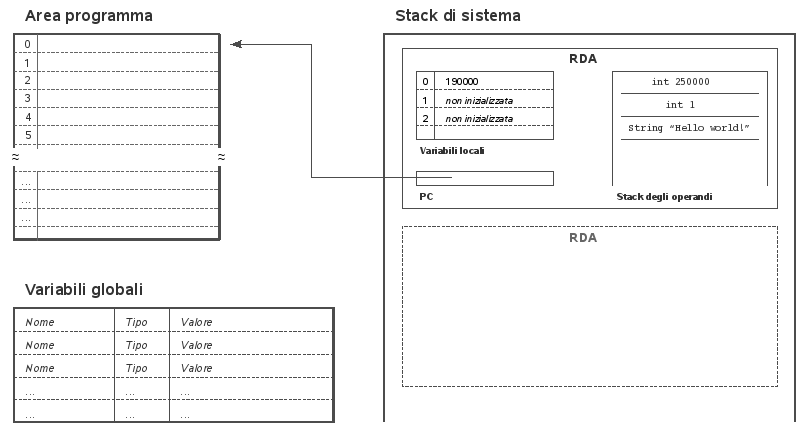
\includegraphics[width=\columnwidth]{graphics/struttura_generale.png}
\end{center}
Nell'\textbf{area programma} ci sono le istruzioni del programma divise in funzioni ed ogni istruzione ha un indice univoco e consecutivo all'istruzione che la precede. Nello spazio \textbf{variabili globali} ci sono tutte le variabili globali con il loro valore, distinte in base al nome e al tipo. Lo \textbf{stack di sistema} contiene i RDA (record di attivazione): ogni funzione ha un suo RDA, una chiamata a funzione comporta l'inserimento di un nuovo RDA sullo \textbf{stack di sistema} e le istruzioni ``return'' tolgono un RDA dallo stack. Ogni RDA ha uno \textbf{stack degli operandi}, uno spazio per le \textbf{variabili locali} e un \textbf{PC} (program counter); lo \textbf{stack degli operandi} viene utilizzato dalle varie istruzioni (vedere il funzionamento delle istruzioni in \ref{sec:dettagli_istruzioni}); lo spazio delle \textbf{variabili locali} contiene fino a 65536 ``registri'' nei quali si possono memorizzare o leggere valori, rispettivamente con le istruzioni ``store'' e ``load''; infine il \textbf{PC} contiene l'indice dell'istruzione da eseguire dell'\textbf{area programma}.

\subsection{Funzionamento}
Vengono eseguiti una serie di passi iniziali per costruire e inizializzare le strutture dati della macchina astratta, dopodich\'e l'esecuzione passa ad una funzione ``esecutore'' che si occupa di eseguire le istruzioni del programma.

\subsubsection*{Inizio}
\begin{enumerate}
  \item Legge il file contenente il programma e carica le istruzioni (divise per funzioni) nella struttura dati \textbf{area programma}.
  \item Ricerca le variabili globali nel programma e le mette nello spazio \textbf{variabili globali}.
  \item Se esiste la funzione \texttt{<clinit>} (funzione per inizializzare le variabili globali) crea un RDA vuoto nello \textbf{stack di sistema}, imposta il PC alla prima istruzione della funzione \texttt{<clinit>}, passa il controllo alla funzione esecutore e, quando ha terminato, prosegue con il punto seguente. Se tale funzione non esiste prosegue con il punto seguente.
  \item Costruisce il primo RDA nello \textbf{stack di sistema} con lo stack degli operandi vuoto, le variabili locali non inizializzate e il PC che punta alla prima istruzione della funzione \texttt{main}.
  \item Passa il controllo all'\textbf{esecutore} che esegue le istruzioni puntate dal PC e termina quando lo \textbf{stack di sistema} \`e vuoto (l'istruzione \texttt{return} toglie un RDA dallo stack).
\end{enumerate}

\subsubsection*{Esecutore}
\begin{enumerate}
  \item Controlla se lo \textbf{stack di sistema} \`e vuoto. Se non \`e vuoto continua, altrimenti termina l'esecuzione.
  \item Prende il valore del PC del RDA in cima allo \textbf{stack di sistema}.
  \item Legge l'istruzione puntata dal PC.
  \item Incrementa il PC.
  \item Esegue l'istruzione seguendo le specifiche in \ref{sec:dettagli_istruzioni}.
  \item Ritorna al punto 1.
\end{enumerate}

%\pagebreak

% IMPLEMENTAZIONE IN C++ *******************************************************
\section{Implementazione in C++}
\label{sec:implementazione}
La macchina astratta \`e stata implementata in C++, definendo e utilizzando le seguenti classi:
\begin{description}
  \item[ActivationRecord:] rappresenta un record di attivazione, con un PC, uno stack degli operandi e un'area per le variabili locali. Fornisce dei metodi per leggere e scrivere nelle variabili locali, per cambiare il valore del PC e per eseguire le operazioni fondamentali (leggere, togliere e mettere un elemento) sullo stack degli operandi.
  \item[SystemStack:] rappresenta uno stack di sistema, praticamente una pila di ActivationRecord. Fornisce dei metodi per inserire e togliere un record di attivazione e per accedere a quello in cima alla pila.
  \item[GlobalVariablesArea:] rappresenta l'area dove vengono memorizzate le variabili globali del programma ed il loro valore. Permette di aggiungere variabili globali e di scriverne e leggere il valore.
  \item[ProgramArea:] in un oggetto di questo tipo viene mantenuto l'insieme delle istruzioni del programma, suddivise per funzione di appartenenza, con un indice univoco associato e consecutivo in modo da poter essere ``puntate'' dal PC di un RdA.
\end{description}
Il programma si compone di due funzioni principali di nome \texttt{main} ed \texttt{esecutore}, mantenute rispettivamente nei file \textit{macchina-astratta.cc} e \textit{esecutore.cc}.\\
Nel file \textit{macchina-astratta.cc} vengono definiti tre oggetti di tipo \texttt{ProgramArea}, \texttt{GlobalVariablesArea} e \texttt{SystemStack} che rappresentano rispettivamente l'\textbf{area programma}, lo spazio per le \textbf{variabili globali} e lo \textbf{stack di sistema}.\\
La funzione \texttt{main} prende come argomento il nome del file da eseguire (contenente il programma), dopodich\`e esegue i seguenti passi:
\begin{enumerate}
  \item Inizializza l'oggetto di tipo \texttt{ProgramArea} e carica le istruzioni del programma al suo interno.
  \item Inizializza l'oggetto di tipo \texttt{GlobalVariablesArea} e ci mette dentro le variabili globali del programma.
  \item Se all'interno del programma da eseguire esiste la funzione ``<clinit> ()V'' (per l'inizializzazione delle variabili globali) crea un record di attivazione vuoto nell'oggetto di tipo \texttt{SystemStack} impostando il PC alla prima istruzione di ``<clinit> ()V'' e chiama la funzione \texttt{esecutore}.
  \item Crea un record di attivazione nell'oggetto di tipo \texttt{SystemStack} e imposta il PC alla prima istruzione della funzione ``main'' del programma da eseguire.
  \item Passa il controllo alla funzione \texttt{esecutore} che si occupa di eseguire le istruzioni contenute nell'oggetto \texttt{ProgramArea}.
\end{enumerate}
La funzione \texttt{esecutore}, finch\`e nell'oggetto \texttt{SystemStack} c'\`e almeno un record di attivazione, esegue i seguenti passi:
\begin{enumerate}
  \item Prende il valore del PC del record di attivazione in cima all'oggetto di tipo \texttt{SystemStack}.
  \item Legge l'istruzione dall'oggetto di tipo \texttt{ProgramArea} "puntata" dal PC.
  \item Incrementa il PC.
  \item Esegue l'istruzione chiamando una funzione appropriata.
\end{enumerate}

\subsection{Compilazione, installazione e documantazione}
Per compilare e creare l'eseguibile della macchina astratta, o per creare la documentazione attraverso doxygen, \`e possibile dare uno dei seguenti comandi all'interno della directory ``macchina-astratta'' dove sono presenti i file sorgente:
\begin{itemize}
  \item \texttt{make}: crea l'eseguibile \texttt{macchina-astratta} dentro la directory ``bin''.
  \item \texttt{make doc}: crea la documentazione del codice in formato html e pdf dentro la directory ``doc''.
\end{itemize}
L'eseguibile \texttt{macchina-astratta} si aspetta come argomento un file, all'interno del quale ci dovr\`a essere il codice del programma da eseguire.

%\pagebreak

% ESEMPI ***********************************************************************
%\section{Esempio}
\label{sec:esempio}
Ecco quindi un semplice esempio di programma eseguibile sulla macchina astratta:



%\pagebreak

% FINE DOCUMENTO ***************************************************************
\end{document}
